%%%%%%%%%%%%%%%%%%%%%%%%%%%%%%%%%%%%%%%%%%%%%%%%%%%%%%%%%%%%%%%%%%%%%%%%%%%%%%%%
%2345678901234567890123456789012345678901234567890123456789012345678901234567890
%        1         2         3         4         5         6         7         8


\documentclass[conference]{IEEEtran}
\usepackage{blindtext, graphicx}
\usepackage{listings}
\lstset { %
    language=C++,
    numbers=left,
    breaklines=true,
    xleftmargin=4em,
    resetmargins=true,
    basicstyle=\footnotesize,
    numberstyle=\footnotesize,
}
\usepackage{graphicx}
\usepackage[font=small]{caption}

%Pacote para acentos [Por TIAGO]
\usepackage[utf8]{inputenc}

% Comment this line out
                                                          % if you need a4paper
%\documentclass[a4paper, 10pt, conference]{ieeeconf}      % Use this line for a4
                                                          % paper

%\IEEEoverridecommandlockouts                              % This command is only
                                                          % needed if you want to
                                                          % use the \thanks command
%\overrideIEEEmargins
% See the \addtolength command later in the file to balance the column lengths
% on the last page of the document



% The following packages can be found on http:\\www.ctan.org
%\usepackage{graphics} % for pdf, bitmapped graphics files
%\usepackage{epsfig} % for postscript graphics files
%\usepackage{mathptmx} % assumes new font selection scheme installed
%\usepackage{times} % assumes new font selection scheme installed
%\usepackage{amsmath} % assumes amsmath package installed
%\usepackage{amssymb}  % assumes amsmath package installed

\title{Impact Analysis of Population Density Growth on Real Estate}

%\author{ \parbox{3 in}{\centering Huibert Kwakernaak*
%         \thanks{*Use the $\backslash$thanks command to put information here}\\
%         Faculty of Electrical Engineering, Mathematics and Computer Science\\
%         University of Twente\\
%         7500 AE Enschede, The Netherlands\\
%         {\tt\small h.kwakernaak@autsubmit.com}}
%         \hspace*{ 0.5 in}
%         \parbox{3 in}{ \centering Pradeep Misra**
%         \thanks{**The footnote marks may be inserted manually}\\
%        Department of Electrical Engineering \\
%         Wright State University\\
%         Dayton, OH 45435, USA\\
%         {\tt\small pmisra@cs.wright.edu}}
%}

% author names and affiliations
% use a multiple column layout for up to three different
% affiliations
\author{\IEEEauthorblockN{D.P.B.S.Gunasekara\IEEEauthorrefmark{1},
C.W.Mohottala\IEEEauthorrefmark{2}, K.P.S.Lakshani\IEEEauthorrefmark{3} and
M.N.K.Gamage\IEEEauthorrefmark{4}}
\IEEEauthorblockA{Department of Computer Science and Engineering,\\
University of Moratuwa\\
Sri Lanka\\
Email: \IEEEauthorrefmark{1}dinelka.gunasekara.19@cse.mrt.ac.lk,
\IEEEauthorrefmark{2}chathuranga.mohottala.19@cse.mrt.ac.lk,\\
\IEEEauthorrefmark{3}shanika.lakshani.19@cse.mrt.ac.lk,
\IEEEauthorrefmark{4}nishshanka.gamage@gmail.com}}

\begin{document}

\maketitle
\thispagestyle{empty}
\pagestyle{empty}


%%%%%%%%%%%%%%%%%%%%%%%%%%%%%%%%%%%%%%%%%%%%%%%%%%%%%%%%%%%%%%%%%%%%%%%%%%%%%%%%
\begin{abstract}

Having a clear visibility on future trends is important in decision making. General public confront the uncertainty when investing on a land, deciding whether it’s wise to do the investment or not. Although statistics are available over decades, proper analysis was not conducted to predict future trends of property rates.\\


Keywords: Population Density, Census, Land Rate, Analysis\\

\end{abstract}


%%%%%%%%%%%%%%%%%%%%%%%%%%%%%%%%%%%%%%%%%%%%%%%%%%%%%%%%%%%%%%%%%%%%%%%%%%%%%%%%
\section{Introduction}

Property rates in Sri Lanka are getting increased year by year in trending rate. This can be due to many reasons. Primarily demand goes high when the supply is limited. Also, that will be influenced by the development of infrastructure facilities. At the same time, it was noted that population density is getting increased with the population growth. The population density growth varies from district to district. Suburb near Colombo city are getting crowded with high population density in recent years.

This research is aimed to understand the correlation between the population density growth and  the increasing trend in property rates in Sri Lanka.\\


\section{Data Collection}

We considered three data sets for the data analysis research study. The first data set is gathered from a prominent real estate website. Statistical data on sales price of houses, apartments and commercial buildings, and residential land price over 8 years from year 2011 to 2018 is obtained. This data represents advertised prices of the land sales from a sample of 15000 property ads. The second data set is gathered from Department of census and statistics, where district population statistics over a century in census years from year 1871 to 2012 is available. In order to calculate the population density of each district / province, a third data-set is taken from the same source which provides land and inland water area of Sri Lanka categorized under district and provincial wise as of year 2012.

Figure \ref{fig:figure3} displays the population density distribution with time over different regions. In order to provide clear visualization, this representation uses logarithmic values of population density.

\begin{figure}
\centering
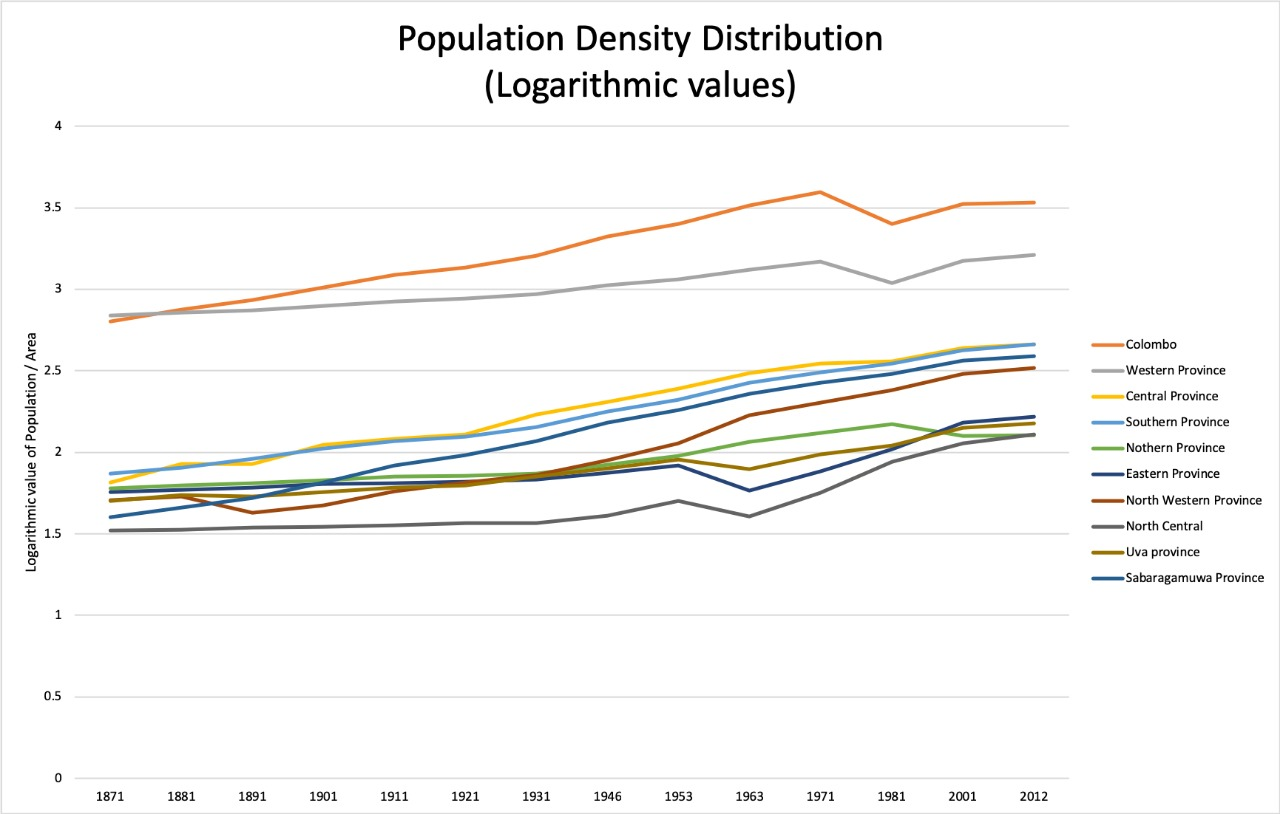
\includegraphics[width=7.5cm]{pop-den-time.jpeg}
\caption{Linear chart representation between Population Density and Time period over different regions}
\label{fig:figure3}
\end{figure}


\section{Methodology}

Our next approach is to process collected data, in a way appropriate for a proper analysis. The population data extracted from government information site was having some empty data points related to some specific past years on some districts. Government could not conduct censuses on those areas due to war and political instability. As the method of handling missing values we have considered a data imputation method rather than data deletion since the available data for the analysis is limited and omitting records would lead to biased results. Since number of data records is limited to carry out time-series specific methods, we replaced those empty data slots with the mean value of particular entry column, as the only dependent factor we are taking is the year. Then these data set is applied in to linear regression model. From that model, predicted population on next five years and expected population from 2011 to 2018 is calculated for all districts and provinces. Using district-wise land area (without the inland water area) of Sri Lanka, population density of each district in each census year is calculated. Here we have assumed that throughout the century, there was no significant change in the provincial area. Using the same linear regression model, population density is estimated for above mentioned periods. 

In the real estate data-set, property price changes over past years ( from 2011 to 2018 ) are available for Colombo district and all nine provinces. Then these data are sub-categorized into residential land prices, cultivation land prices, property rental and sales prices.

Spearman correlation coefficient with each of these data set is calculated against above estimated population density  data-set to see the relationship between each data-set with the population density. 


\section{Analysis}

The data analysis is mainly categorized into three theoretical techniques. Linear Regression with Time Series Analysis, Data Extrapolation & Correlation Analysis. 

Population Density Growth is modeled as Linear Regression Time Series. Since we have past data from 1871 the most appropriate modeling technique is the Linear Regression model. Using this model will facilitate forecast the future Population Density growth for every district.

Extrapolation technique is used to draw missing data points for the land price data set.
Correlation Analysis technique is used to compare two Linear Regression model for the Population Density and Land Price Trend.


\subsection{Analysis of population density on residential land price}

According to the calculated Pearson’s correlation coefficients between population density and residential land price shown in Table \ref{table_1}, in Colombo region and Western province are having the highest correlation of more than 0.9. Therefore we can conclude that the residential land prices in western province are highly impacted from population density growth over time. 

North western province (Kurunegala District and Puttalam District) is having a correlation of 0.8, where the impact on residential land price is not affected by population density growth as western province, but has some considerable effect on it. All the other provinces are having low correlation value where there are more other factors effect on residential land prices other than population density growth. 

The distribution of population density and residential land prices over time over various regions are plotted in Figure\ref{fig:figure1}. 

\begin{table}[h]
\caption{Correlation between Population Density and Residential Land Price}
\label{table_1}
\begin{center}
\begin{tabular}{|l|c|}
\hline
\textbf{Region} & \textbf{Correlation}\\
\hline
Western Province & 0.9157\\
\hline
Colombo & 0.9031\\
\hline
North Western Province & 0.8187\\
\hline
North Central Province & 0.5911\\
\hline
Sabaragamuwa Province & 0.3802\\
\hline
Southern Province & 0.2516\\
\hline
Uva Province & 0.1760\\
\hline
Central Province & 0.1759\\
\hline
Eastern Province & 0.0938\\
\hline
Nothern Province & -0.3666\\
\hline
\end{tabular}
\end{center}
\end{table}

%O mesmo voce pode fazer para citar a Figura \ref{fig:g1.jpeg}.

\begin{figure}
\centering
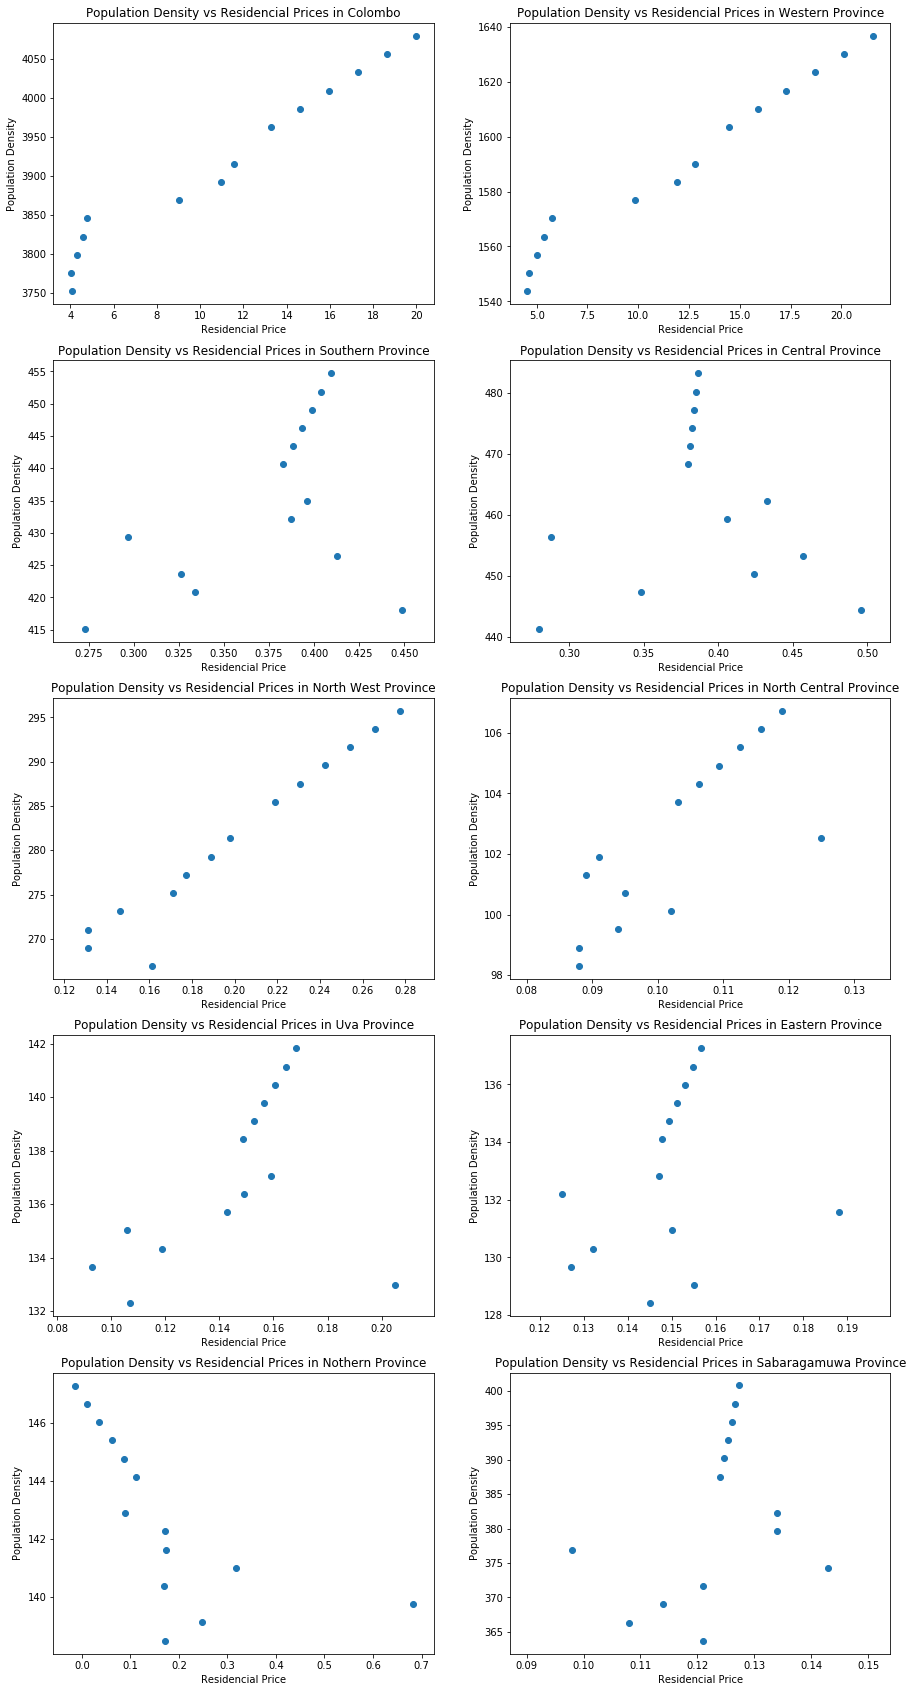
\includegraphics[width=9.25cm]{pop-den-res-price.png}
\caption{Scatter Plot between Population Density and Residential Land Prices over different regions}
\label{fig:figure1}
\end{figure}


\subsection{Analysis of Population Density on Property Rental Price}

According to the calculated correlation data on Table \ref{table_2}, colombo region house rental prices have very high correction with population density growth. Every other house rental and apartment rental prices in other provinces are having significantly low correlation between population density growth. 

\begin{table}[h]
\caption{Correlation between Population Density and Property Rental Price}
\label{table_2}
\begin{center}
\begin{tabular}{|l|c|}
\hline
\textbf{Property} & \textbf{Correlation}\\
\hline
Colombo House Rental price & 0.9227\\
\hline
Western Province (except Colombo) House Rental price & 0.5386\\
\hline
North West province House Rental price & 0.1830\\
\hline
Colombo Apartment Rental price & 0.1566\\
\hline
Central province House Rental price & -0.2928\\
\hline
Southern province House Rental price & -0.4066\\

\hline
\end{tabular}
\end{center}
\end{table}

%O mesmo voce pode fazer para citar a Figura \ref{fig:pop-den-rent-price.jpeg}.

\begin{figure}
\centering
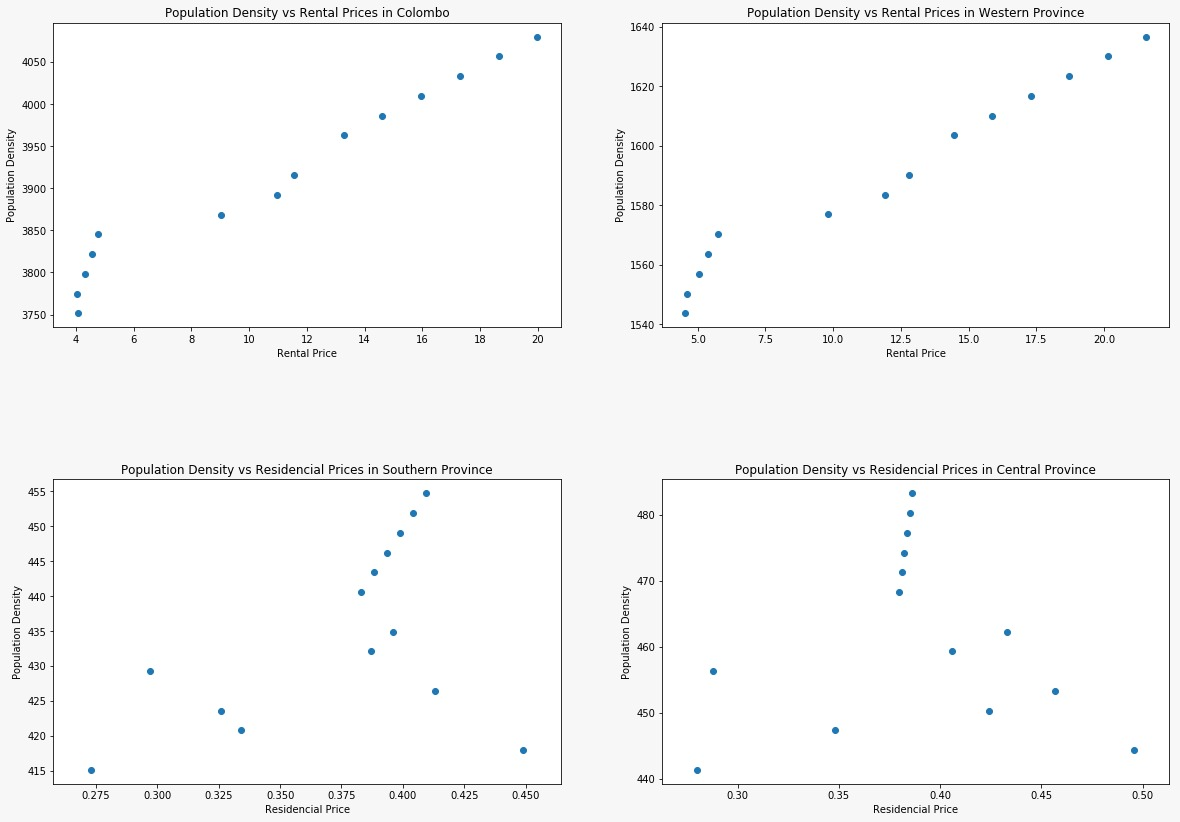
\includegraphics[width=9cm]{pop-den-rent-price.jpeg}
\caption{Scatter Plot between Population Density and Property Rental Prices over different regions}
\label{fig:figure2}
\end{figure}


\subsection{Analysis of Population Density on Property Sale Prices}

According to the calculated correlation data on Table \ref{table_3} western province houses, apartments and commercial buildings sales prices having high correlation to population density. 

\begin{table}[h]
\caption{Correlation between Population Density and Property Sale Price}
\label{table_3}
\begin{center}
\begin{tabular}{|l|c|}
\hline
\textbf{Property} & \textbf{Correlation}\\
\hline
Western Province (except Colombo) House & 0.9662\\
\hline
Colombo Apartment & 0.9634\\
\hline
Central Province House & 0.8747\\
\hline
Colombo House & 0.8739\\
\hline
Colombo Commercial Buildings & 0.7825\\
\hline
North West Province House & 0.6918\\
\hline
Southern Province House & 0.5122\\
\hline
Sabaragamuwa Province House & 0.4129\\
\hline
Uva Province House & -0.0315\\
\hline
North Central Province House & -0.0588\\
\hline
Eastern Province House & -0.0642\\
\hline
Northern Province House & -0.4543\\
\hline
\end{tabular}
\end{center}
\end{table}


\section{Conclusion And Discussion}

Research was able to identify the there is a linear correlation between the population density and the Residential Prices in Western Province and North West Province. Also especially in Colombo district the correlation between Population Density Vs Residential Price was + 0.9. It was not prominent this correlation in other provinces in Sri Lanka. When the population density increases the correlation between the residential prices make visible in linear regression.

It was also noted that there was an exceptional increase in AVG Price/perch in Colombo district starting from 2015. 

This model can be used to predict future population density and how that is going to impact to the residential prices. The current data set is only limited to Colombo in district level and other areas in provincial level. In order to come up with more insightful predictions data must be collected and analyzed for fine grained Geo-locations  like suburb and villages.


\addtolength{\textheight}{-12cm}   % This command serves to balance the column lengths
                                  % on the last page of the document manually. It shortens
                                  % the textheight of the last page by a suitable amount.
                                  % This command does not take effect until the next page
                                  % so it should come on the page before the last. Make
                                  % sure that you do not shorten the textheight too much.

%%%%%%%%%%%%%%%%%%%%%%%%%%%%%%%%%%%%%%%%%%%%%%%%%%%%%%%%%%%%%%%%%%%%%%%%%%%%%%%%

\bibliographystyle{IEEEtran}

 
\bibliography{IEEEexample}
% \bibitem{latexcompanion} 
% Michel Goossens, Frank Mittelbach, and Alexander Samarin. 
% \textit{The \LaTeX\ Companion}. 
% Addison-Wesley, Reading, Massachusetts, 1993.
 
% \bibitem{einstein} 
% Albert Einstein. 
% \textit{Zur Elektrodynamik bewegter K{\"o}rper}. (German) 
% [\textit{On the electrodynamics of moving bodies}]. 
% Annalen der Physik, 322(10):891–921, 1905.

\end{document}
